% !TeX program = lualatex
% !BIB program = biber
% Lualatex is important to render TTF fonts; with pdflatex it's just the regular one
% ratio 16:9 -- https://tex.stackexchange.com/questions/14336/

% compile two versions, inspired by https://tex.stackexchange.com/a/1501
% use the script "compile-pdf.sh"
\newif\ifhandout
% if flags.tex does not exist, create an empty file to be able to compile in TeXstudio
\input{flags}

\ifhandout
\documentclass[12pt,aspectratio=169,handout]{beamer}
\else
\documentclass[12pt,aspectratio=169]{beamer}
\fi



% TODO change "leftfootertext" to your liking
\newcommand{\leftfootertext}{\insertsubtitle}  % just the \title{} text by default
%\newcommand{\leftfootertext}{RNNs and encoder-decoder architectures}  % Your name, for instance


% ------- RUB specifics ----------
% adjust for 16:9
% https://tex.stackexchange.com/questions/354022/modifying-the-margins-of-all-slides-in-beamer
\setbeamersize{text margin left=0.3cm,text margin right=4.5cm} 


% use Metropolis as the basis theme
\usetheme[subsectionpage=progressbar]{metropolis}
% blocks with background globally
\metroset{block=fill}


\usepackage{fontspec}
% RUB fonts need to be installed
% 'UprightFont = * Light' makes sure that the base font is RubFlama Light, which looks
% lighter than RubFlama Regular (would be too thick for slides)
\setsansfont[Scale=MatchLowercase, UprightFont = * Light, BoldFont = * Bold]{RubFlama}
%\setsansfont{Arial} % Open source alternative if you don't have RubFlama

% RUB color scheme
% Dark blue: 0; 53; 96; #003560
\definecolor{RUBDarkBlue}{RGB}{0, 53, 96}

% Light yellow (table fill, etc.); 238; 250; 196; #EEFAC4
\definecolor{RUBLightYellow}{RGB}{238, 250, 196}

%Light green: 141; 174; 16
\definecolor{RUBLightGreen}{RGB}{141, 174, 16}


\setbeamercolor{titlelike}{fg=RUBDarkBlue}
\setbeamercolor{subtitle}{fg=RUBLightGreen}
\setbeamercolor{separation line}{fg=RUBLightGreen}
\setbeamercolor{frametitle}{bg=white, fg=RUBDarkBlue}

% horizontal line on title page and sections
\setbeamercolor{alerted text}{fg=RUBLightGreen}


% Adjust footer bottom (too large by default)
\setbeamertemplate{footline}{%
  \begin{beamercolorbox}[wd=\textwidth, sep=2ex]{footline}%
    \usebeamerfont{page number in head/foot}%
    \usebeamertemplate*{frame footer}
    \hfill%
    \usebeamertemplate*{frame numbering}
  \end{beamercolorbox}%
}


% Lab name, numbering, etc. in footer
\setbeamertemplate{frame numbering}{TrustHLT --- Prof.\ Dr.\ Ivan Habernal \hspace*{1ex} 
\includegraphics[width=7em]{img/rub-logo.pdf}\hspace*{1ex}}

\setbeamertemplate{frame footer}{\hspace*{1ex}\insertframenumber \hspace*{2ex} \leftfootertext}

% adjust the background to be completely white
\setbeamercolor{background canvas}{bg=white}

% logos on the title page
\titlegraphic{%
	\begin{picture}(0,0)
		\put(435,0){\makebox(0,0)[rt]{
\includegraphics[width=7em]{img/rub-logo.pdf}}}
		\put(435,-170){\makebox(0,0)[rt]{
\includegraphics[width=4em]{img/logo-trusthlt.pdf}}}
		\put(435,-196){\makebox(0,0)[rt]{
\includegraphics[width=9em]{img/logo-rctrust.pdf}}}
	\end{picture}%
}


% show TOC at every section start
\AtBeginSection{
	\frame{
		\vspace{2em}
		\sectionpage
		\hspace*{2.2em}\begin{minipage}{10cm}
			\tableofcontents[currentsection]
		\end{minipage}
	}
}

% TOC without subsection
\setcounter{tocdepth}{1} % only-- part,chapters,sections 

% bullet points: rectangles
\useinnertheme{rectangles}
\setbeamercolor{itemize item}{fg=RUBLightGreen}
\setbeamercolor{itemize subitem}{fg=RUBLightGreen}
% enumerate: blue background for better readability
\setbeamercolor{item projected}{bg=RUBDarkBlue}

% make boxes (example, block, etc.) background lighter for readability
\setbeamercolor{block title}{%
	use=normal text,
	fg=normal text.fg,
	bg=normal text.bg!90!fg % lighter background in block title
}
\setbeamercolor{block body}{
	use={block title, normal text},
	bg=block title.bg!30!normal text.bg % lighter background in block body
}


% RUB colors in blocks
\setbeamercolor{block title alerted}{%
	use={block title, alerted text},
	bg=RUBDarkBlue,
	%fg=RUBLightYellow % looks bad
	fg=white % better contrast
}

\setbeamercolor{block title example}{%
	use={block title, example text},
	fg=RUBLightGreen
}


% ------- end of RUB specifics ----------

% all itemize with pause by default
%\beamerdefaultoverlayspecification{<+->}


% typeset mathematics on serif
\usefonttheme[onlymath]{serif}

% better bibliography using biber as backend
\usepackage[natbib=true,backend=biber,style=authoryear-icomp,maxbibnames=30,maxcitenames=9,uniquelist=false,giveninits=true,doi=false,url=false,dashed=false,isbn=false]{biblatex}
% shared bibliography
\addbibresource{../../nlpwdl-bibliography.bib}
% disable "ibid" for repeated citations
\boolfalse{citetracker}



\usepackage{xspace}


% for derivatives, https://tex.stackexchange.com/a/412442
\usepackage{physics}

\usepackage{tikz}
\usetikzlibrary{matrix, positioning}
\usetikzlibrary{angles,quotes} % for angles
\usetikzlibrary{backgrounds} % background
\usetikzlibrary{decorations.pathreplacing} % curly braces
\usetikzlibrary{calligraphy}
\usetikzlibrary{calc} % for neural nets

% for plotting functions
\usepackage{pgfplots}
\usepgfplotslibrary{dateplot}

% sub-figures
\usepackage{caption}
\usepackage{subcaption}

% book tabs
\usepackage{booktabs}


% argmin, argmax
\usepackage{amsmath}
\DeclareMathOperator*{\argmax}{arg\!\max}
\DeclareMathOperator*{\argmin}{arg\!\min}
% softmax
\DeclareMathOperator*{\softmax}{soft\!\max}
% Mask
\DeclareMathOperator*{\mask}{mask}

% bold math
\usepackage{bm}

% for \mathclap
\usepackage{mathtools}

% algorithms
\usepackage[noend]{algpseudocode}


% for neurons and layers in tikz
\tikzset{
	neuron/.style={draw, rectangle, inner sep=2pt, minimum width=0.75cm, fill=blue!20},
	param/.style={draw, rectangle, inner sep=2pt, minimum width=0.75cm, fill=green!20},
	constant/.style={draw, rectangle, inner sep=2pt, minimum width=0.75cm, fill=black!15},
	% for citation nodes right top
	ref/.style={anchor = north east, text width=7.8cm, yshift=-1.3cm, xshift=-0.2cm, scale=0.5},
	state/.style={rectangle, inner sep=2pt, minimum width=0.75cm, fill=black!5},
}

% added in lecture 10
\tikzset{
	mtx/.style={
		matrix of math nodes,
		left delimiter={[}, right delimiter={]}
	},
	hlt/.style={opacity=0.1, line width=4 mm, line cap=round},
	hltr/.style={opacity=0.5, rounded corners=2pt, inner sep=-1pt}
}

% for strike-through text (added in Lecture 06)
\usepackage[normalem]{ulem}

% added in Lecture 7
% RNN
\DeclareMathOperator*{\rnn}{RNN}
% RNN star
\DeclareMathOperator*{\rnnstar}{RNN^{*}}
% bi-RNN
\DeclareMathOperator*{\birnn}{biRNN}


% added in Lecture 9
\usetikzlibrary{fit} % for hightligting by calling "fit"

% algorithms
\usepackage[noend]{algpseudocode}



\title{Natural Language Processing with Deep Learning}
\subtitle{Lecture 1 --- NLP tasks and evaluation}
\date{October 16, 2025}
\author{Prof.\ Dr.\ Ivan Habernal}
\institute{
\texttt{www.trusthlt.org} \\
Trustworthy Human Language Technologies Group (TrustHLT) \\
Ruhr University Bochum \& Research Center Trustworthy Data Science and Security}



\begin{document}

\maketitle


%\begin{frame}{Table of contents}
%\setbeamertemplate{section in toc}[sections numbered]
%\tableofcontents[hideallsubsections]
%\end{frame}



\section{Motivation}

\begin{frame}{Why study deep learning for NLP?}

\pause
\begin{enumerate}
\item Build another AI startup and get filthy rich
\item Get the skill-set to destroy Skynet, if that happens
\end{enumerate}
\bigskip

\pause
But maybe also: Research on safety \& security of LLMs, privacy, fairness, agentic AI, green AI, domain-specific LLMs, etc.

\end{frame}

% shrink size
\begin{frame}[shrink=20]{Preliminary course roadmap}

\begin{enumerate}
	\item NLP tasks and evaluation
	\item Mathematical foundations of deep learning
	\item Text classification 1: Log-linear models
	\item Text classification 2: Deep neural networks
	\item Text generation 1: LMs and word embeddings
	\item Text classification 3: Encoding with RNNs
	\item Text generation 2: Autoregressive RNNs and attention
	\item Text classification 4: Self-attention and BERT
	\item Text generation 3: Transformers
	\item Text generation 4: Decoder-only models and GPT
	\item Contemporary LLMs: Prompting and in-context learning
	\item To be continued
\end{enumerate}


	
\end{frame}

\section{Course logistics}


\begin{frame}{Lecturers and tutors}

Lecturers\footnote{\url{ivan.habernal@ruhr-uni-bochum.de}}

\begin{itemize}
	\item Prof.\ Dr.\ Ivan Habernal
\end{itemize}

Exercise tutors

\begin{itemize}
	\item also me
\end{itemize}

\end{frame}



\begin{frame}{Online resources}
	
\begin{itemize}
	\item Moodle for homework, announcements, and forum: \url{https://moodle.ruhr-uni-bochum.de/course/view.php?id=66993}
	\item GitHub for lectures: \url{https://github.com/trusthlt/nlp-with-deep-learning-lectures}
	\item Discord as much faster forum: To be announced at Moodle
	\item Lectures recorded and published on YouTube
\end{itemize}
	
\end{frame}

\begin{frame}{Textbooks and resources}
	
\begin{itemize}
	\item Recommended for each topic or lecture separately
	\item We'll use freely available resources (almost exclusively)
\end{itemize}

Top-notch research in NLP is "open source"

\begin{itemize}
	\item Association for Computational Linguistics (ACL) conferences in the "Anthology": \url{https://aclanthology.org/}
	\item \url{https://arXiv.org}
\end{itemize}
	
\end{frame}



\begin{frame}{Exercises}
	
\begin{itemize}
	\item Deepen your understanding of the matter, mostly hands-on
	\item Not graded
	\item We provide a guide-book and the assignment (mostly code, sometimes paper \& pen)
\end{itemize}


\end{frame}

\begin{frame}{Final exam}
	
	
\begin{itemize}
\item February 11, 2026
\item E-Assessment-Center in GAFO 04/402
\item Exam questions: En
\item Answers: En or De
\end{itemize}

\end{frame}



\begin{frame}{It's your course, too!}
	
Your feedback is very important

\begin{itemize}
	\item Talk to me (live, discord, forum, e-mail)
	\item I'll post anonymous feedback forms regularly
	\item Slides issues: Just open bug/PR on GitHub
\end{itemize}


\end{frame}



\begin{frame}{TrustHLT --- Trustworthy Human Language Technologies}
	


\begin{block}{Research focus}
\begin{itemize}
	
	\item Privacy-preserving NLP (differential privacy; deep learning; representation learning; anonymization)	
	\item Legal NLP, legal argumentation
	
\end{itemize}	
\end{block}


	\bigskip
	
	Master thesis? HiWi job? Get in touch!
	
	\url{ivan.habernal@ruhr-uni-bochum.de}
	
\end{frame}




\section{Challenges of NLP}

\begin{frame}{Ambiguity and variability of human language}
	
	
	\begin{example}[Highly ambiguous]
		Compare ``I ate pizza with friends'' to ``I ate pizza with olives''
	\end{example}
	
	
	
	\begin{example}[Highly variable]
		The core message of ``I ate pizza with friends'' can be expressed as
		``friends and I shared some pizza''
	\end{example}
	
	Humans --- great users of language, very poor at formally understanding and describing rules that govern language
	
	
	\begin{tikzpicture}[overlay, remember picture] 
		\node at (current page.north east)[ref] {\fullcite{Goldberg.2017} \par};
	\end{tikzpicture}	
	
\end{frame}




%\begin{frame}{Supervised machine learning to save us...}
%	
%	The best known set of methods for dealing with language data $\to$ supervised machine learning algorithms
%	\begin{itemize}
%		\item ML attempts to infer patterns and regularities from a set of pre-annotated input--output pairs
%		\item ML excels at problem domains where a good set of rules is very hard to
%		define but annotating the expected output for a given input is relatively simple
%	\end{itemize}
%	
%\end{frame}


\begin{frame}{Language is challenging for machine learning (ML)}
	
	Natural language exhibits properties that make it very challenging for ML
	
	\begin{enumerate}
		\item Discrete
		\item Compositional
		\item Sparse
	\end{enumerate}
	
\end{frame}

\begin{frame}{Language is symbolic and discrete}
	
	Basic elements of written language: \textbf{characters}
	
	Characters form \textbf{words} that denote objects, concepts, events, actions, and ideas
	
	\begin{block}{Characters and words are discrete symbols}
		\begin{itemize}
			\item Words such as ``hamburger'' or ``pizza'' each evoke in us a certain mental representations
			\item But they are distinct symbols, whose meaning is external to them, to be interpreted in our heads
			\item No inherent relation between ``hamburger'' and ``pizza'' can be inferred from the symbols or letters themselves
		\end{itemize}
	\end{block}
	
\end{frame}

\begin{frame}{Characters and words are discrete symbols}
	
	Compare that to concepts such as \textbf{color} (in machine vision), or acoustic
	signals --- these concepts are \textbf{continuous}
	
	\begin{itemize}
		\item Colorful image to gray-scale image using a simple mathematical operation
		\item We can compare two different colors based on inherent properties such as hue and intensity
	\end{itemize}
	
	\begin{block}{This cannot be easily done with words}
		There is no simple operation to move from the word ``red'' to the word ``pink'' without using a large lookup table or a dictionary
	\end{block}
	
\end{frame}


\begin{frame}{Language is compositional}
	Letters $\to$ words $\to$ phrases $\to$ sentences
	
	The meaning of a phrase can be larger than the meaning of the individual words,	and follows a set of intricate rules
	
	\begin{example}
		Multi-word expressions (``New York'', ``look something up'') \\
		Idioms (``kick the bucket'', ``blue chip'')
	\end{example}
	
	To interpret a text, we need to work beyond the level of letters and words, and look at long sequences of words such as sentences, or even complete documents
\end{frame}


\begin{frame}{Data sparseness}
	
	Combinations of words to form meanings $\to \infty$
	
	\begin{itemize}
		\item We could never enumerate all possible valid sentences
	\end{itemize}
	
	
	No clear way of generalizing from one sentence to another, or defining the similarity between sentences, that does not depend on their meaning which is unobserved to us
	
	
	\begin{block}{Challenging when learning from examples}
		Even with a huge example set we are very likely to observe events that never occurred in the example set and that are very different
	\end{block}
	
\end{frame}




\section{Overview of typical NLP tasks}


\begin{frame}{Why are we learning this?}
	
Important question to ask before we even start!

\bigskip

Deep learning is a tool and we need to understand

\begin{itemize}
	\item Why we need this tool in the first place
	\item How do we know we have the right tool (it's doing its job well)
\end{itemize}


\end{frame}


\begin{frame}{Coarse typology}
Text classification and text generation
\end{frame}

\subsection{Text classification tasks}

\begin{frame}{ Sentiment classification of movie reviews}

Binary classification of reviews from IMDB

\begin{example}
	\textbf{Text:} Read the book, forget the movie! \\
	\textbf{Label:} Negative
\end{example}	

$\to$ semantic compositionality, long-range dependencies

\begin{tikzpicture}[overlay, remember picture] 
\node at (current page.north east)[ref] {\fullcite{Maas.et.al.2011} \par};
\end{tikzpicture}

\begin{itemize}
\item IMDB is the MNIST of NLP (the limus paper), 25k training, 25k test data points, balanced
\item Why was it interesting?
\end{itemize}

\end{frame}

\begin{frame}{ Task and dataset are used as synonyms}

``The IMDB dataset" --- must be properly cited! (incl.\ link)

\begin{block}{Where to get datasets?}
\url{https://huggingface.co/datasets}

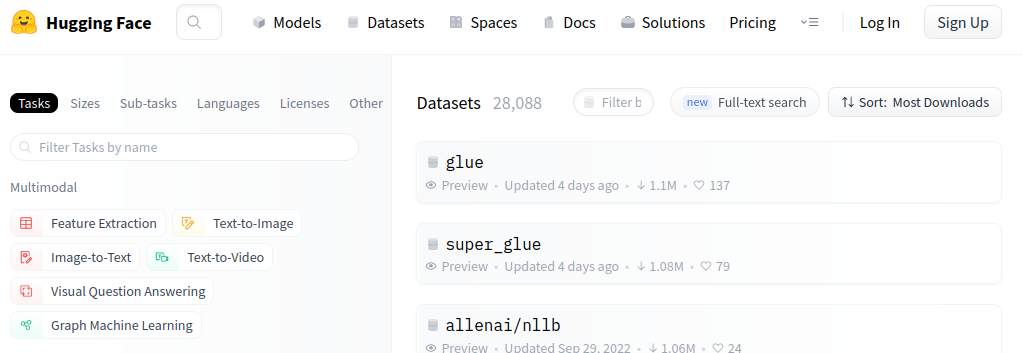
\includegraphics[width=0.97\linewidth]{img/hfdata.png}
\end{block}

\end{frame}

\begin{frame}{Natural Language Inference}

Two sentences: entailment, contradiction, or neutral?

\begin{example}
\textbf{Text:} A soccer game with multiple males playing. \\
\textbf{Hypothesis:} Some men are playing sport. \\
\textbf{Label:} Entailment
\end{example}


The ``standard" NLI paper and dataset from Stanford: SNLI

\begin{itemize}
	\item 570k human-written English sentence pairs
\end{itemize}

How is SNLI data different from the IMDB?

\begin{itemize}
	\item IMDB data that was ``annotated for free" by each author
\end{itemize}


\begin{tikzpicture}[overlay, remember picture] 
\node at (current page.north east)[ref] {\fullcite{Bowman.et.al.2015} \par};
\end{tikzpicture}

\end{frame}

\begin{frame}{Side step 1: Gold standard data}

\begin{itemize}
	\item Many datasets are annotated by experts, super costly
	\item Each example by multiple annotators, then the final ``gold" label is decided upon
\end{itemize}

\bigskip

How to measure task subjectivity and annotation quality?

\begin{block}{Inter-Annotator Agreement}
Take chance agreement into account
\begin{itemize}
	\item Cohen's Kappa, Scott's Pi, Krippendorff's Alpha, Krippendorff's Unitized Alpha \citep{Artstein.Poesio.2008.CoLi}
\end{itemize}
	
\end{block}


\begin{tikzpicture}[overlay, remember picture] 
\node at (current page.north east)[ref] {\fullcite{Habernal.et.al.2023.AILaw} 
\bigskip \newline	
\fullcite{Artstein.Poesio.2008.CoLi} \par};
\end{tikzpicture}
\end{frame}



\begin{frame}{ Side step 2: Who creates these tasks and why?}

\begin{itemize}
	\item Mostly researchers
	\item Mostly for phenomena in language and to which extent NLP can ``solve" them
	\item Shared datasets became popular with machine learning in NLP
\end{itemize}

Tasks are classified into various (arbitrary) taxonomies with (mostly agreed upon) names, for example

\begin{itemize}
	\item Sentiment analysis $\in$ text classification
	\item SNLI $\in$ sentence-pair classification
\end{itemize}


\end{frame}

\begin{frame}[fragile]{ Deeper in sentences: NER}

Named entity recognition: Find entities of predefined types

\begin{example}
\begin{verbatim}
 U.N.         Organization
 official     
 Ekeus        Person
 heads        
 for          
 Baghdat      Location
 .            
\end{verbatim}
\end{example}

How to model and annotate such a task?

\begin{tikzpicture}[overlay, remember picture] 
	\node at (current page.north east)[ref] {\fullcite{TjongKimSang.DeMeulder.2003} \par};
\end{tikzpicture}

\end{frame}

\begin{frame}[fragile]{NER: Sequence labeling task}

Tokenize, assign each word a type

\begin{example}
\begin{verbatim}
 U.N.         I-ORG
 official     O
 Ekeus        I-PER
 heads        O
 for          O
 Baghdat      I-LOC
 .            O
\end{verbatim}
\end{example}

CoNLL 2003: Four entities (PER, ORG, LOC, MISC)

\begin{tikzpicture}[overlay, remember picture] 
\node at (current page.north east)[ref] {\fullcite{TjongKimSang.DeMeulder.2003} \par};
\end{tikzpicture}
\end{frame}



\begin{frame}[fragile]{NER: BIO encoding}
	
What if two consequent tokens are same type?

\bigskip
	
\begin{quote}
``Whenever two entities of type XXX are immediately next to each other, the first word of the second entity will be tagged B-XXX in order to show that it starts another entity''
\end{quote}


BIO encoding

\bigskip

An instance of Multi-class classification on token level

\begin{tikzpicture}[overlay, remember picture] 
\node at (current page.north east)[ref] {\fullcite{TjongKimSang.DeMeulder.2003} \par};
\end{tikzpicture}	
\end{frame}



\begin{frame}{SuperGLUE}
	
SuperGLUE --- popular benchmark collection of various tasks/datasets in English
	
%	SuperGLUE We use a subset of the SuperGLUE (Wang et al., 2019) evaluation suite of classification tasks, specifically:

\bigskip

\begin{quote}
``The goal of SuperGLUE is to provide a simple, robust evaluation metric of any method capable of being applied to a broad range of \textbf{language understanding} tasks.''
\end{quote}
	
%In BLOOM:
%Ax-b, Ax-g, BoolQ, CB, WiC, WSC, and RTE tasks.
	

\begin{tikzpicture}[overlay, remember picture] 
	\node at (current page.north east)[ref] {\fullcite{Wang.et.al.2019.NeurIPS} \par};
\end{tikzpicture}
	
\end{frame}

%\begin{frame}{Recognizing Textual Entailment (RTE)}
%	
%	Two-class (binary) classification
%	
%	Whether or not the Text entails the Hypothesis
%	
%	\begin{example}
%		\textbf{Text:} Dana Reeve, the widow of the actor Christopher Reeve, has died of lung cancer at age 44, according to the Christopher Reeve Foundation. \\
%		\textbf{Hypothesis:} Christopher Reeve had an accident. \\
%		\textbf{Entailment:} False
%	\end{example}
%	
%	\begin{tikzpicture}[overlay, remember picture] 
%		\node at (current page.north east)[ref] {\fullcite{Dagan.et.al.2009.NLE} \par};
%	\end{tikzpicture}
%	
%
%Note: SNLI adapted RTE!
%	
%\end{frame}


%\begin{frame}{Coreference resolution (WSC --- Winograd Schema\\ Challenge)}
%	
%	Examples consist of a sentence with a pronoun and a list of noun phrases from the sentence
%	
%	Determine the correct referrent of the pronoun
%	
%	\begin{example}
%		\textbf{Text:} Mark told \underline{Pete} many lies about himself, which Pete included in his book. \underline{He} should have been more truthful.
%		
%		\textbf{Coreference:} False
%	\end{example}	
%	
%	$\to$ everyday knowledge and commonsense reasoning to solve
%	
%	\begin{tikzpicture}[overlay, remember picture] 
%		\node at (current page.north east)[ref] {\fullcite{Levesque.et.al.2012} \par};
%	\end{tikzpicture}
%	
%\end{frame}

%
%\begin{frame}{BoolQ}
%	
%Each example: short passage and a yes/no question about the passage
%
%\begin{example}
%Q: Has the UK been hit by a hurricane? \\
%P: The Great Storm of 1987 was a violent extratropical cyclone which caused casualties in England, France and the Channel Islands ... \\
%A: Yes. [An example event is given.]
%\end{example}
%	
%$\to$ complex, non-factoid information, requires difficult entailment-like inference to solve
%
%\begin{tikzpicture}[overlay, remember picture] 
%\node at (current page.north east)[ref] {\fullcite{Clark.et.al.2019.NAACL} \par};
%\end{tikzpicture}
%
%\end{frame}


%
%\begin{frame}{MultiRC: Multi-Sentence Reading Comprehension}
%
%Each example consists of
%\begin{itemize}
%	\item Context paragraph
%	\item Question about that paragraph
%	\item List of possible answers (true/false)
%\end{itemize}
%
%Desirable properties:
%\begin{enumerate}
%	\item Multiple possible correct answers $\to$ each question-answer pair must be evaluated independent of other pairs
%	\item Answering each question requires drawing facts from multiple context sentences
%\end{enumerate}
%
%
%\begin{tikzpicture}[overlay, remember picture] 
%\node at (current page.north east)[ref] {\fullcite{Khashabi.et.al.2018.NAACL} \par};
%\end{tikzpicture}
%
%\end{frame}

\begin{frame}{Extractive Question Answering: SQuAD 2.0}
	
\begin{scriptsize}
\begin{example}
Endangered Species Act Paragraph: ``... Other legislation followed, including the Migratory Bird Conservation Act of 1929, a \textbf{1937 treaty} prohibiting the hunting ofright and gray whales, and the \underline{Bald Eagle Protection Act of 1940}. These \underline{later laws} had a low cost to society---the species were relatively rare---and little \textbf{opposition} was raised."

Question 1: ``Which laws faced significant \textbf{opposition}?" \\
Plausible Answer: \underline{later laws}

Question 2: ``What was the name ofthe \textbf{1937 treaty}?" \\
Plausible Answer: \underline{Bald Eagle Protection Act}
\end{example}
\end{scriptsize}

Unanswerable questions w/ plausible (but incorrect) answers. Relevant keywords are \textbf{bold}.

	
\begin{tikzpicture}[overlay, remember picture] 
\node at (current page.north east)[ref] { \fullcite{Rajpurkar.et.al.2018.ACL} \par};
\end{tikzpicture}
	
\end{frame}


\subsection{Text generation tasks}


\begin{frame}{Machine translation}


\includegraphics[width=13em]{img/mtex.jpg}

Standard datasets from WMT (formerly Workshop on MT)


\begin{tikzpicture}[overlay, remember picture]
\node at (current page.north east)[ref] { \fullcite{Bojar.et.al.2018.WMT} \par};
\end{tikzpicture}

\end{frame}


\begin{frame}{Machine translation}
	

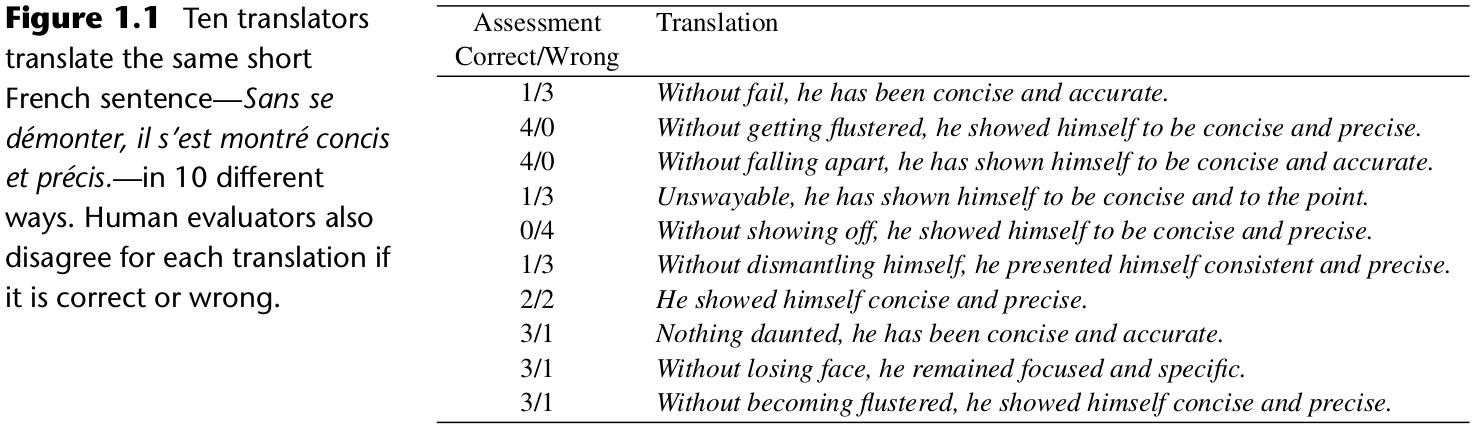
\includegraphics[width=15cm]{img/mt2.png}
	
	
Source: \fullcite{Koehn.2020}
	
\end{frame}


\begin{frame}{(Abstractive) Document summarization}

Popular dataset: CNN/Daily Mail

\begin{itemize}
	\item Online news articles (781 tokens on average)
	\item Paired with multi-sentence summaries (3.75 sentences or 56 tokens on average)
	\item 287k training pairs, 13k validation pairs, 11k test pairs
\end{itemize}

\begin{tikzpicture}[overlay, remember picture] 
\node at (current page.north east)[ref] {\fullcite{Hermann.et.al.2015.NeurIPS} \par};
\end{tikzpicture}

\end{frame}

\begin{frame}{Dialogue: PersonaChat}
	
165k utterances; Task: next utterance prediction
	
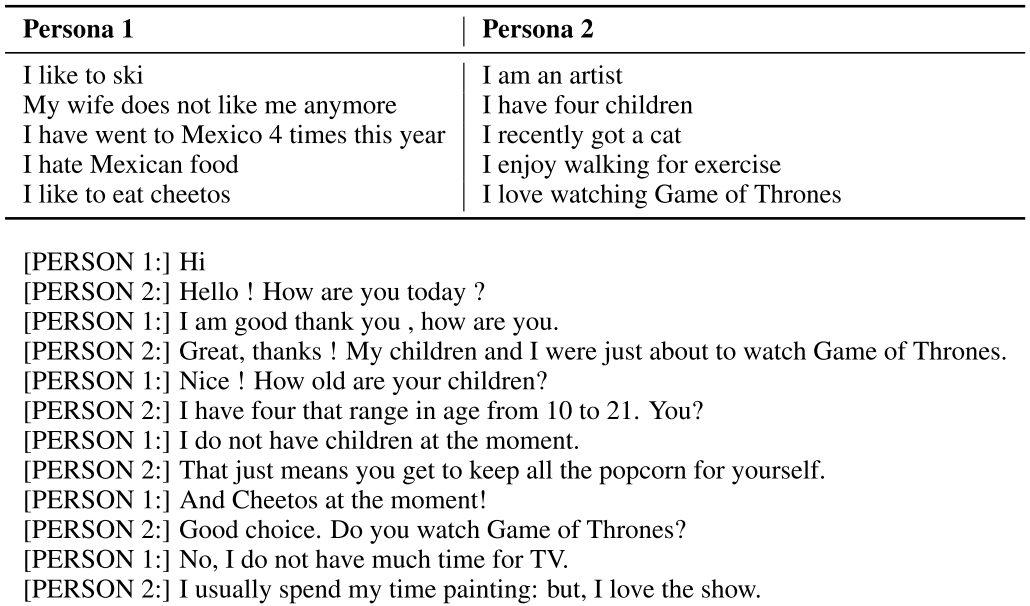
\includegraphics[width=0.9\linewidth]{img/dial1.png}

\begin{tikzpicture}[overlay, remember picture] 
\node at (current page.north east)[ref] {\fullcite{Zhang.et.al.2018.ACL} \par};
\end{tikzpicture}

\end{frame}

\begin{frame}{Overview of some typical generation tasks}

\begin{table}
\begin{footnotesize}
\begin{tabular}{p{5cm}p{6cm}l}
\toprule
NLG task & Context (Input) & Reference \\
\midrule
Machine Translation (MT) & Source language sentence & Translation \\ 
Abstractive Summarization (AS) & Document & Summary \\
Question Answering (QA) & Question + Background info (Passage, Image, etc) & Answer \\
Question Generation (QG) & Passage, Knowledge base, Image & Question \\
Dialogue Generation (DG) & Conversation history & Response \\
Image Captioning (IC) & Image & Caption \\
Data to Text (D2T) & Semi-structured data (Tables, Graphs) & Description \\
\bottomrule
\end{tabular}
\end{footnotesize}
\caption{Context and references for NLG tasks}
\end{table}



\begin{tikzpicture}[overlay, remember picture] 
\node at (15.5, 9.7)[ref] {\fullcite{Sai.et.al.2023.CSUR} \par};
\end{tikzpicture}

\end{frame}


\subsection{Classification as generation}

\begin{frame}{Unifying classification and generation}

Any task incl.\ classification $\to$ "text-to-text" format

\begin{example}[Translation En-De]
Input: \emph{translate English to German: That is good.} \\
Expected output text: \emph{Das ist gut.}
\end{example}

\begin{example}[MNLI]
Input: \emph{mnli premise: I hate pigeons. hypothesis: My feelings towards pigeons are filled with animosity.}
Expected output text: \emph{entailment}
\end{example}

\begin{tikzpicture}[overlay, remember picture] 
\node at (current page.north east)[ref] {\fullcite{Raffel.et.al.2020.JMLR} \par};
\end{tikzpicture}

\end{frame}



\section{Evaluation}


\begin{frame}{ Train/Dev/Test data splits}

Training and Test data

Development (Validation) set used for optimizing hyper-parameters

\tikzstyle{box} = [rectangle, draw, black, text width=3cm]
\tikzstyle{train} = [fill=blue!10]
\tikzstyle{dev} = [fill=yellow!10]
\tikzstyle{test} = [fill=red!10]

\begin{figure}

\begin{tikzpicture}[node distance=0.8cm]
	\node (f13) [box, train] {Train};
	\node (f14) [box, dev, below of=f13] {Validation};
	\node (f15) [box, test, below of=f14] {Test};
	
\end{tikzpicture}

\end{figure}

\end{frame}

%
%\begin{frame}{Cross validation}
%
%\textbf{K-fold cross-validation} partitions the data into $K$ chunks
%
%$K - 1$ of which form the training set $\mathcal{R}$
%
%The last chunk serves as the test set $\mathcal{V}$ (or validation)
%
%\bigskip
%
%\tikzstyle{box} = [rectangle, draw, black, text width=1.5cm]
%\tikzstyle{train} = [fill=blue!10]
%\tikzstyle{test} = [fill=red!10]
%
%\begin{figure}
%	\begin{scriptsize}
%		\begin{tikzpicture}[node distance=0.5cm]
%			\node (f10) [] {Fold 1};
%			\node (f11) [box, train, below of=f10] {Train};
%			\node (f12) [box, train, below of=f11] {Train};
%			\node (f13) [box, train, below of=f12] {Train};
%			\node (f14) [box, train, below of=f13] {Train};
%			\node (f15) [box, test, below of=f14] {Test};
%			
%			\node (f20) [right=1.6cm, right of=f10] {Fold 2};
%			\node (f21) [box, train, below of=f20] {Train};
%			\node (f22) [box, train, below of=f21] {Train};
%			\node (f23) [box, train, below of=f22] {Train};
%			\node (f24) [box, test, below of=f23] {Test};
%			\node (f25) [box, train, below of=f24] {Train};
%			
%			\node (f30) [right=1.6cm, right of=f20] {Fold 3};
%			\node (f31) [box, train, below of=f30] {Train};
%			\node (f32) [box, train, below of=f31] {Train};
%			\node (f33) [box, test, below of=f32] {Test};
%			\node (f34) [box, train, below of=f33] {Train};
%			\node (f35) [box, train, below of=f34] {Train};
%			
%			\node (f40) [right=1.6cm, right of=f30] {Fold 4};
%			\node (f41) [box, train, below of=f40] {Train};
%			\node (f42) [box, test, below of=f41] {Test};
%			\node (f43) [box, train, below of=f42] {Train};
%			\node (f44) [box, train, below of=f43] {Train};
%			\node (f45) [box, train, below of=f44] {Train};
%			
%			\node (f50) [right=1.6cm, right of=f40] {Fold 5};
%			\node (f51) [box, test, below of=f50] {Test};
%			\node (f52) [box, train, below of=f51] {Train};
%			\node (f53) [box, train, below of=f52] {Train};
%			\node (f54) [box, train, below of=f53] {Train};
%			\node (f55) [box, train, below of=f54] {Train};
%		\end{tikzpicture}
%	\end{scriptsize}
%	\caption{Example of 5-fold CV}
%\end{figure}
%
%\end{frame}

\subsection{Evaluation of text classification}


\begin{frame}{Confusion matrix (binary case)}

Two classes: Positive and Negative

\begin{block}{Confusion matrix}
\begin{tabular}{l|cc}
& Predicted Neg & Predicted Pos \\ \toprule
Actually Neg & True negative (TN) & False positive (FP) \\
Actually Pos & False negative (FN) & True positive (TP) \\
\end{tabular}
\end{block}

\bigskip


Ordering of columns and rows is \textbf{arbitrary}!

\end{frame}


\begin{frame}{Accuracy}

Accuracy of classifier $f$ on test set $T$:
$$
\mathrm{Acc}_T(f) = \frac{1}{|T|} \sum_{i = 1}^{|T|} I (f(x_i) = y_i)
$$
	
\begin{example}[Disease detection]
	\begin{tabular}{l|rr}
		& Pred. Negative & Pred. Positive \\ \toprule
		Act. Negative & 168 & 33 \\
		Act. Positive & 48 & 37 \\
	\end{tabular}
\end{example}

$37 + 48 + 33 + 168 = 286$ $\to$ Test set size $|T| = 286$
$\mathrm{Acc}_T(f) = \frac{1}{286} (37 + 168) = 0.7186$

\begin{tikzpicture}[overlay, remember picture] 
\node at (current page.north east)[ref] {\fullcite{Japkowicz.Shah.2011} \par};
\end{tikzpicture}
	
\end{frame}


\begin{frame}{Precision, recall, F-1 score}
	
\begin{block}{Confusion matrix}
	\begin{tabular}{l|cc}
		& Pred. Negative & Pred. Positive \\ \toprule
		Act. Negative & True negative (TN) & False positive (FP) \\
		Act. Positive & False negative (FN) & True positive (TP) \\
	\end{tabular}
\end{block}
	
Precision (for class positive) = TP / (TP + FP)

Recall (for class positive) = TP / (TP + FN)

F-1 score (for class positive) = 2PR / (P + R)
	
\end{frame}


\begin{frame}{Confusion matrix -- multi-class}
	
\begin{tabular}{r|rrrrrrr}
	& prediction: &\rotatebox{90}{\emph{money-fx}}&\rotatebox{90}{\emph{trade}}&\rotatebox{90}{\emph{interest}}&\rotatebox{90}{\emph{wheat}}&\rotatebox{90}{\emph{corn}}&\rotatebox{90}{\emph{grain}}\\
	true class:&&&&&&&\\\hline
	\emph{money-fx} && 95 & 0 & 10 & 0 & 0 & 0\\
	\emph{trade} && 1 & 1 & 90 & 0 & 1 & 0\\
	\emph{interest} && 13 & 0 & 0 & 0 & 0 & 0\\
	\emph{wheat} && 0 & 0 & 1 & 34 & 3 & 7\\
	\emph{corn} && 1 & 0 & 2 & 13 & 26 & 5\\
	\emph{grain} && 0 & 0 & 2 & 14 & 5 & 10
\end{tabular}
	
\end{frame}


\begin{frame}{Confusion matrix --- multi-class}

\begin{itemize}
\item We can unambiguously compute Precision and Recall for each class
\item How to get the F-1 score for the complete test set across classes?
\begin{itemize}
\item Macro-averaging (average of F-1 scores), or micro-averaging
\item These details might get tricky so always report exactly what you do!
\end{itemize}

\end{itemize}
\begin{tikzpicture}[overlay, remember picture] 
\node at (current page.north east)[ref] {\fullcite{Sokolova.Lapalme.2009} \par};
\end{tikzpicture}

\end{frame}















\subsection{Evaluation of text generation}




\begin{frame}{Evaluating text generation is hard}
	
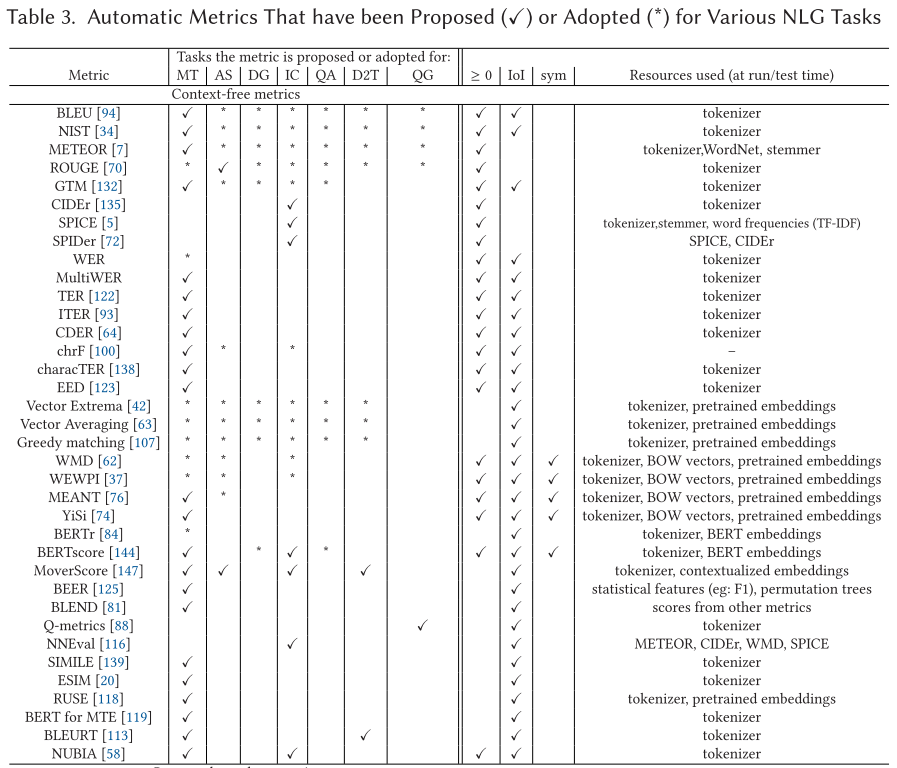
\includegraphics[trim={0 12.2cm 0 0},clip,width=1.2\linewidth]{img/nlg2.png}

\begin{tikzpicture}[overlay, remember picture] 
\node at (15.5, 9.7)[ref] {\fullcite{Sai.et.al.2023.CSUR} \par};
\end{tikzpicture}


\end{frame}


\begin{frame}{BLEU (Bilingual Evaluation Understudy)}

Almost first and most popular metric for MT

\begin{itemize}
	\item Precision-based metric that computes the n-gram overlap between the reference and the hypothesis
	\item In particular, BLEU is the ratio of the number of overlapping n-grams to the total number of n-grams in the hypothesis.
\end{itemize}


Corpus-level metric, i.e., BLEU gives a score over the entire corpus (as opposed to scoring individual sentences)

Major drawbacks of BLEU: (i) it does not take recall into account and (ii) it only allows exact n-gram matching

\begin{tikzpicture}[overlay, remember picture] 
\node at (current page.north east)[ref] {\fullcite{Papineni.et.al.2002.ACL} \par};
\end{tikzpicture}

\end{frame}


\begin{frame}{ROUGE (Recall-Oriented Understudy\\ for Gisting Evaluation)}
	
ROUGE metric includes a set of variants: ROUGE-N, ROUGE-L, ROUGE-W, and ROUGE-S

\begin{itemize}
	\item ROUGE-N is similar to BLEU-N in counting the n-gram matches between the hypothesis and reference, however, it is a recall-based measure unlike BLEU which is precision-based
	\item ROUGE-L measures the longest common subsequence (LCS) between a pair of sentences	
\end{itemize}

\begin{tikzpicture}[overlay, remember picture] 
	\node at (current page.north east)[ref] {\fullcite{Lin.2004} \par};
\end{tikzpicture}


\end{frame}



\subsection{Caveats of NLP benchmarking}


\begin{frame}{Is BLEU a good metric?}

BLEU was originally proposed for diagnostic evaluations of MT systems, that is, as a technique for allowing researchers and developers to quickly ``weed out bad ideas from good ideas''

\begin{itemize}
\item Wide range of correlations between BLEU and human evaluations
\item BLEU should not be the primary evaluation technique in NLP papers
\end{itemize}

\begin{tikzpicture}[overlay, remember picture] 
	\node at (current page.north east)[ref] {\fullcite{Reiter.2018.CoLi} \par};
\end{tikzpicture}


\end{frame}


\begin{frame}{The `gold' data paradigm might not always fit}

The assumption of a ground truth makes sense when humans highly agree on the answer

\begin{itemize}
	\item ``Does this image contain a bird?"
	\item ``Is `learn' a verb?"
	\item ``What is the capital of Italy?"
\end{itemize}

This assumption often does not make sense, especially when language is involved

\begin{itemize}
	\item ``Is this comment toxic?"
\end{itemize}

\emph{Human label variation impacts all steps of the traditional ML pipeline, and is an opportunity, not a problem}

\begin{tikzpicture}[overlay, remember picture] 
	\node at (current page.north east)[ref] {\fullcite{Plank.2022.EMNLP} \par};
\end{tikzpicture}

\end{frame}




\begin{frame}{New and new benchmarks...}



\begin{figure}
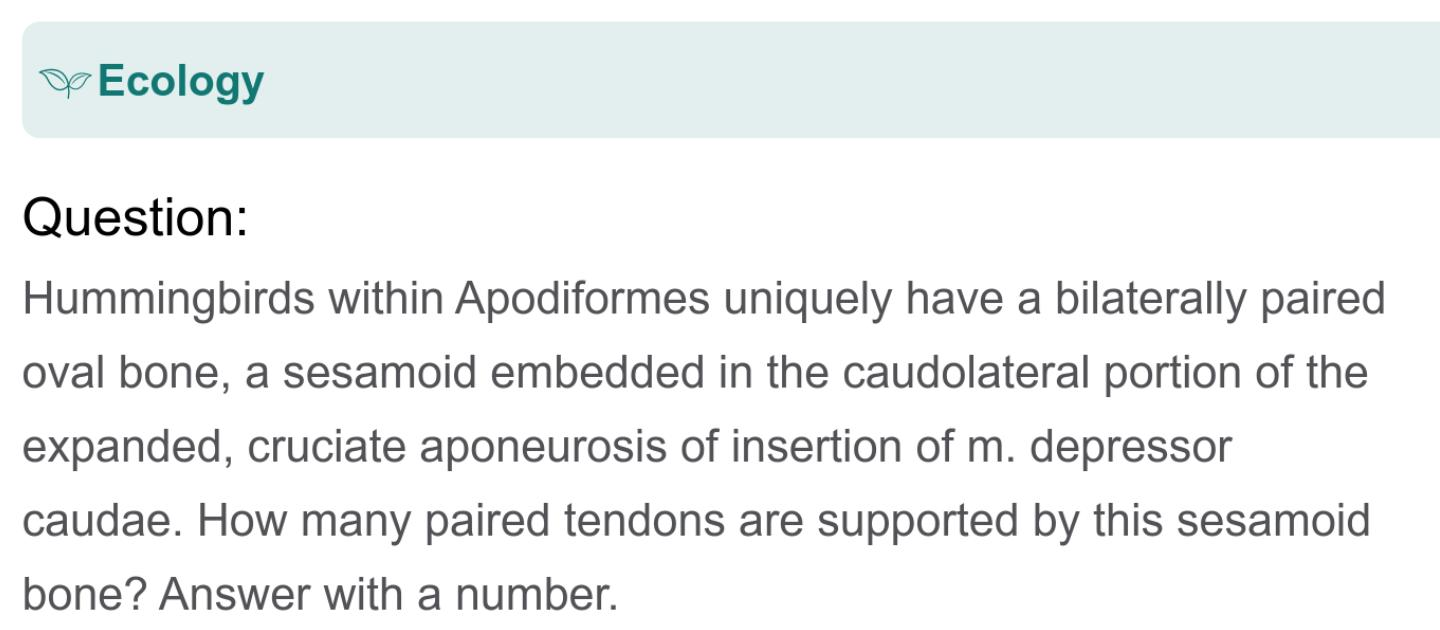
\includegraphics[width=0.8\linewidth]{img/humanity2.jpg}
\caption{Example from the Humanity's Last Exam dataset. The benchmark contains 2,500 challenging questions across over a hundred subjects.}
\end{figure}

\begin{tikzpicture}[overlay, remember picture] 
	\node at (current page.north east)[ref] {\fullcite{phanHumanitysLastExam2025} \par};
\end{tikzpicture}

\end{frame}


\begin{frame}{But performance of LLMs keeps rising}
\begin{figure}
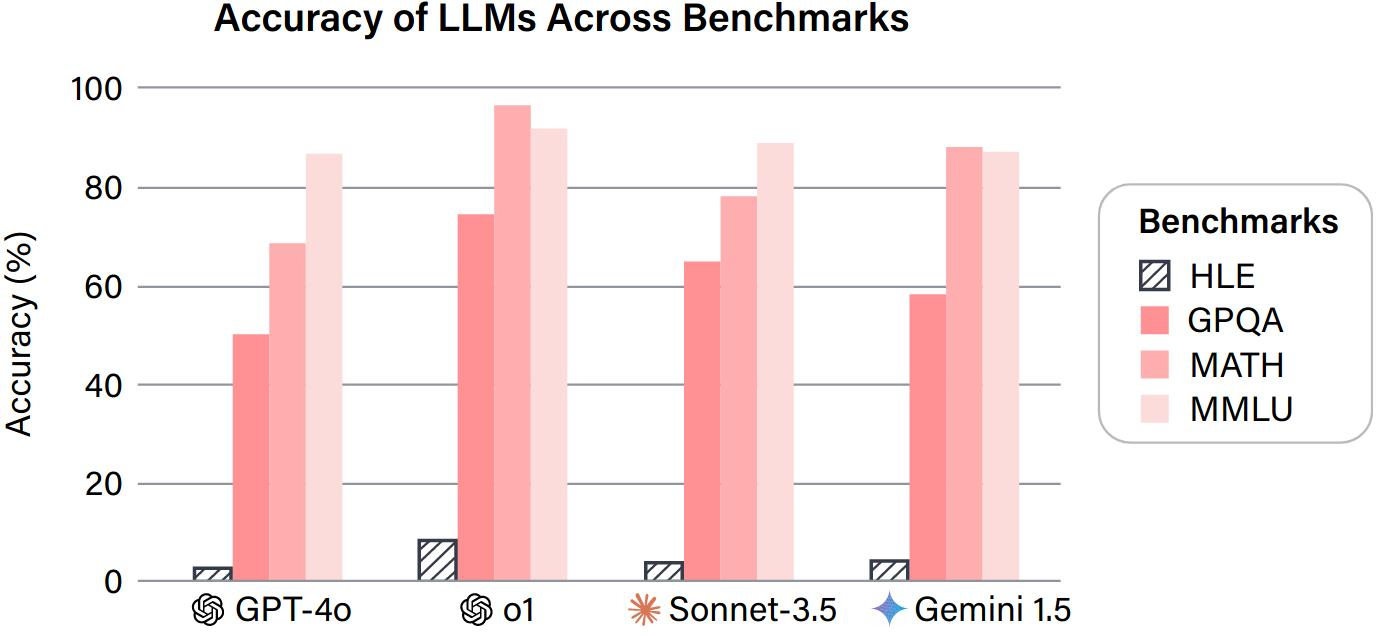
\includegraphics[width=\linewidth]{img/humanitylastexam.jpg}
\end{figure}


\begin{tikzpicture}[overlay, remember picture] 
	\node at (current page.north east)[ref] {\fullcite{phanHumanitysLastExam2025} \par};
\end{tikzpicture}

\end{frame}



\begin{frame}{Beware of (unintended) data contamination!}

Data contamination = evaluate LLMs on the same data they were trained on

\bigskip

\begin{quote}
``90 papers accessed ChatGPT through the web interface, hence providing data that OpenAI could have used to further improve its models''
\end{quote}

\begin{tikzpicture}[overlay, remember picture] 
	\node at (current page.north east)[ref] {\fullcite{Balloccu.et.al.2024.EACL} \par};
\end{tikzpicture}

\end{frame}


%\begin{frame}{ Human annotators are biased}
%
%Datasets are often constructed using a small number of annotators, and humans are biased
%
%\begin{itemize}
%	\item Concerns about data diversity, especially when workers freely generate sentences
%	\item Models do not generalize well to examples from annotators that did not contribute to the training set
%\end{itemize}
%
%\begin{tikzpicture}[overlay, remember picture] 
%	\node at (current page.north east)[ref] {\fullcite{Geva.et.al.2019.EMNLP} \par};
%\end{tikzpicture}
%
%\end{frame} \begin{frame}{Artifacts in datasets}
%
%Datasets have artifacts (spurious statistics) that can be exploited
%
%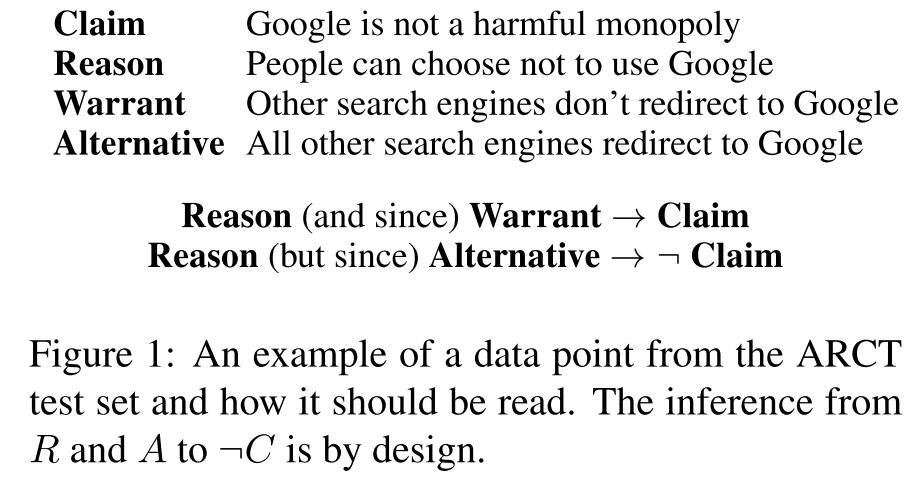
\includegraphics[width=8cm]{img/arct.png}
%
%
%
%\begin{tikzpicture}[overlay, remember picture] 
%	\node at (current page.north east)[ref] {\fullcite{Habernal.et.al.2018.NAACL.ARCT} 
%		\bigskip \newline	
%		\fullcite{Niven.Kao.2019.ACL} \par};
%\end{tikzpicture}
%
%
%\end{frame}


\section*{Recap}

\begin{frame}{Takeaways: We set up the scene}
	
\begin{itemize}
	\item NLP is challenging
	\item Vast amount of tasks and datasets
	\item Data quality matters
	\item Understanding the data, annotators, task matters too
	\item Deep familiarity with common evaluation metrics is essential
	\item Getting better scores is just a beginning of the story
	\item Evaluating generation is an art
\end{itemize}
	
\end{frame}



\begin{frame}{License and credits}

	\begin{columns}
		\begin{column}{0.7\textwidth}
			Licensed under Creative Commons Attribution-ShareAlike 4.0 International (CC BY-SA 4.0)
		\end{column}
		\begin{column}{0.2\textwidth}
			
\includegraphics[width=0.9\linewidth]{img/cc-by-sa-icon.pdf}
		\end{column}
	\end{columns}
	
	\bigskip
	
	Credits
	
	\begin{scriptsize}
		
		Ivan Habernal
		
		Content from ACL Anthology papers licensed under CC-BY \url{https://www.aclweb.org/anthology}
		
	\end{scriptsize}
	
\end{frame}



\end{document}

